\documentclass[a4 paper]{article}
% Set target color model to RGB
\usepackage[inner=1.5cm,outer=1.5cm,top=2.5cm,bottom=2.5cm]{geometry}
\usepackage{setspace}
\usepackage[rgb]{xcolor}
\usepackage{verbatim}
\usepackage{amsgen,amsmath,amstext,amsbsy,amsopn,tikz,amssymb,tkz-linknodes}
\usepackage{fancyhdr}
\usepackage[colorlinks=true, urlcolor=blue,  linkcolor=blue, citecolor=blue]{hyperref}
\usepackage[colorinlistoftodos]{todonotes}
\usepackage{rotating}
%\usetikzlibrary{through,backgrounds}
\hypersetup{%
pdfauthor={Arman Shokrollahi},%
pdftitle={Homework},%
pdfkeywords={Tikz,latex,bootstrap,uncertaintes},%
pdfcreator={PDFLaTeX},%
pdfproducer={PDFLaTeX},%
}
%\usetikzlibrary{shadows}
\usepackage[francais]{babel}
\usepackage{booktabs}
\newcommand{\ra}[1]{\renewcommand{\arraystretch}{#1}}

      \newtheorem{thm}{Theorem}[section]
      \newtheorem{prop}[thm]{Proposition}
      \newtheorem{lem}[thm]{Lemma}
      \newtheorem{cor}[thm]{Corollary}
      \newtheorem{defn}[thm]{Definition}
      \newtheorem{rem}[thm]{Remark}
      \numberwithin{equation}{section}

\newcommand{\homework}[6]{
   \pagestyle{myheadings}
   \thispagestyle{plain}
   \newpage
   \setcounter{page}{1}
   \noindent
   \begin{center}
   \framebox{
      \vbox{\vspace{2mm}
    \hbox to 6.28in { {\bf\hfill} }
       \vspace{6mm}
       \hbox to 6.28in { {\Large \hfill #1 (#2)  \hfill} }
       \vspace{6mm}
       \hbox to 6.28in { {\it Instructor: #3 \hfill Student: #5} }
       %\hbox to 6.28in { {\it TA: #4  \hfill #6}}
      \vspace{2mm}}
   }
   \end{center}
   \markboth{#5 -- #1}{#5 -- #1}
   \vspace*{4mm}
}

\newcommand{\bbF}{\mathbb{F}}
\newcommand{\bbX}{\mathbb{X}}
\newcommand{\bI}{\mathbf{I}}
\newcommand{\bX}{\mathbf{X}}
\newcommand{\bY}{\mathbf{Y}}
\newcommand{\bepsilon}{\boldsymbol{\epsilon}}
\newcommand{\balpha}{\boldsymbol{\alpha}}
\newcommand{\bbeta}{\boldsymbol{\beta}}
\newcommand{\0}{\mathbf{0}}

\begin{document}
\homework{Actividad \#9}{Aproximaci\'on al c\'alculo del periodo del p\'endulo}{Carlos Liz\'arraga Celaya}{}{Antonio Cota Rodr\'iguez}{}

\section*{Introducci\'on}

La integraci\'on de la ecuaci\'on del movimiento, sin la aproximaci\'on de pequeñas oscilaciones, es considerablemente m\'as complicada e involucra integrales el\'ipticas de primera especie, para el periodo de un p\'ndulo simple de amplitud arbitraria tenemos:

$$T = 4 \cdot \sqrt{\frac{l}{2g}}\int_{0}^{\theta_{0}}\frac{1}{\sqrt{\cos{\theta}-\cos{\theta_{0}}}}d\theta $$

La integral diverge a medida que $\theta_{0}$ tiende a la vertical.\\

La integral se puede escribir como una integral el\'iptica de primer tipo, obteniendo la expresi\'on:

$$ T = 4 \cdot \sqrt{\frac{l}{g}}K\left(\sin^{2}{\left(\frac{\theta_{0}}{2}\right)}\right) $$

as\'i $K$ es

$$K(k) = F\left(\frac{\pi}{2},k\right) = \int_{0}^{\pi/2}\frac{1}{\sqrt{1-k^{2}\sin^{2}{u}}}du $$

donde F es la integral el\'iptica completa de primera especie. La integral el\'iptica puede ser aproximada por una serie de potencias descrita por la expresión:

$$K(k) = \frac{\pi}{2}\left[1 + \left(\frac{1}{2}\right)^{2}k^{2} + \left(\frac{1 \cdot 3}{2 \cdot 4}\right)^{2}k^{4} +...+ \left[\frac{(2n-1)!!}{(2n)!!}\right]^{2}k^{2n}+...\right]$$

La soluci\'on exacta del periodo del p\'endulo es:

$$T(\theta) = 2\pi \sqrt{\frac{l}{g}} \left[1 + \left(\frac{1}{2}\right)^{2}\sin^{2}{\frac{\theta_{0}}{2}} + \left(\frac{1 \cdot 3}{2 \cdot 4}\right)^{2}\sin^{4}{\frac{\theta_{0}}{2}} + \left(\frac{1 \cdot 3 \cdot 5}{2 \cdot 4 \cdot 6}\right)^{2}\sin^{6}{\frac{\theta_{0}}{2}}+...\right] $$


o en forma de suma:

$$ T(\theta) = 2\pi \sqrt{\frac{l}{g}}\left[\sum_{n=0}^{\infty}\left(\frac{(2n)!}{2^{n}(n!)^{2}}\right)^{2}\sin^{2n}{\left(\frac{\theta_{0}}{2}\right)}\right]$$

donde $\theta$, es la amplitud angular. Así pues, el periodo es función de la amplitud de las oscilaciones.

En la presente actividad reproduciremos la gr\'afica que aparece en la pr\'actica 9 en la cual se represental la inclusi\'on de 2 hasta 10 t\'erminos de la serie de potencias.\\

Despu\'es se aplicar\'a una serie de Maclaurin.

\section{Programa}

En ipython se utilizó el siguiente c\'odigo para representar los 10 t\'erminos de la serie de potencias:

\begin{verbatim}
import numpy as np
from scipy import integrate
import matplotlib.pyplot as plt
import math

t=100
n=6
x=[]
TT0_0=[]
TT0=[]
x_0=np.linspace(0.001,np.pi + 0.001, t)

I = lambda x,a: 1/np.sqrt(np.cos(x) - np.cos(a))

for i in range(t):
#   la integral
    theta_0=x_0[i]
    T_0 , err= integrate.quad(I, 0, theta_0, args=(theta_0,))
    
    
#   Periodo
    TT0_0.append((4/np.sqrt(2)) * T_0)

    
#  Ciclos   
for v in range(n):
    
#   Error   
    err=[]
        
    for i in range(t):
    
    
        theta_0 = x_0[i]
        T0=1

#   SUMA     
        for u in range(v):
            
            T0 += math.pow( math.factorial(2*(u+1)) / (math.pow( math.pow(2,(u+1)) * math.factorial(u+1) , 2 ) ) , 2 ) * math.pow( np.sin(theta_0 / 2), 2*(u+1) )   
            
#   Lista de errores          
        err.append(100*(np.absolute(2 * np.pi * T0 - TT0_0[i])/TT0_0[i]))
   
#   GRÁFICA   
    plt.plot(x_0 * 180 / np.pi, err, '-.', linewidth=2, label='$T %i $' % (2*v))
    
    

   
#   DESVIACIÓN
plt.title('Errores relativos de las series de potencias')
plt.xlabel(r'$ \theta _0 (deg)$')
plt.ylabel("Error Relativo (%)")
plt.xlim(0,120)
plt.ylim(0,1)
plt.xticks(np.arange(0,130,10))
plt.yticks(np.arange(0,1.1,0.1))
plt.legend(loc='center left', bbox_to_anchor=(1, 0.5))
plt.grid()
plt.show()


Err=[]
for i in range(t):
    theta_0 = x_0[i]
    T0=1
    for u in range(80):
        sen=0
# Maclaurin
        for k in range(80):
            sen += math.pow(-1,k)/math.factorial(2*k+1) * math.pow(theta_0/2, 2*k+1)
            
        T0 += math.pow( math.factorial(2*(u+1)) / (math.pow( math.pow(2,(u+1)) * math.factorial(u+1) , 2 ) ) , 2 ) * math.pow( sen , 2*(u+1) )   
    
    Err.append(100*(np.absolute(2 * np.pi * T0 - TT0_0[i])/TT0_0[i]))

plt.plot(x_0 * 180 / np.pi, Err, '-.',color='k', linewidth=2, label='$T %i $' % (2*v))
plt.title('Error usando serie de Maclaurin')
plt.xlabel(r'$ \theta _0 (deg)$')
plt.ylabel("Error Relativo (%)")
plt.xlim(0,180)
plt.ylim(0,1)
plt.xticks(np.arange(0,190,10))
plt.yticks(np.arange(0,1.1,0.1))
plt.legend(loc='center left', bbox_to_anchor=(1, 0.5))
plt.grid()
plt.show()

\end{verbatim}

Las gr\'aficas que nos imprimi\'o el c\'odigo fueron las siguientes.

\begin{figure}[!ht]
  \centering
      \includegraphics[width=10cm, height=6cm]{Terminos.png}
  \caption{}
\end{figure}
\newpage
\begin{figure}[!ht]
  \centering
      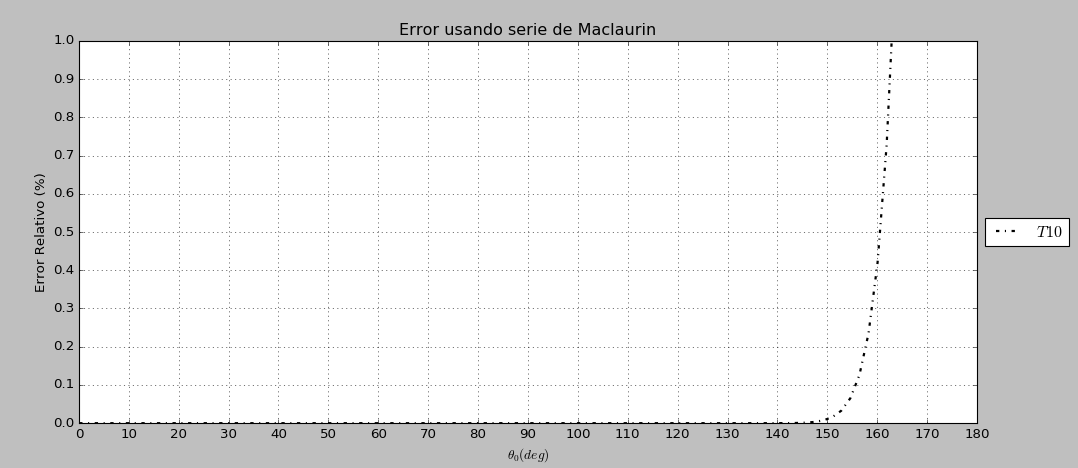
\includegraphics[width=10cm, height=6cm]{Maclaurin.png}
  \caption{}
\end{figure}

\section*{Conclusiones}

En esta pr\'actica aprendimos a utilizar mejor el comando {\it scipy.integrate} no present\'o mucha dificultad, y si se obtuvieron las gr\'aficas deseadas.



\end{document}